\documentclass{beamer}

\usepackage[utf8]{inputenc}
\usepackage[T1]{fontenc}
\usepackage[ruled,vlined,linesnumbered]{algorithm2e}
\usepackage{tikz}

\usepackage{verbatim}
\usetikzlibrary{arrows,shapes}

\SetAlFnt{\small}
\SetAlCapFnt{\large}
\SetAlCapNameFnt{\large}

%%% algorithm2e environment with "Algoritmi"-caption.
\newenvironment{finalgo}[1][htb]{
  \renewcommand{\algorithmcfname}{Algoritmi}
  \begin{algorithm}[#1]
}{\end{algorithm}}

%%% To be able to not numbering individual lines:
\let\oldnl\nl% Store \nl in \oldnl
\newcommand{\nonl}{\renewcommand{\nl}{\let\nl\oldnl}}

%%% argmin
\DeclareMathOperator*{\argmin}{arg\, min}

\title{{\rmfamily\scshape Lyhimpien polkujen hakualgoritmit ja -järjestelmät}}
\author{$\mathfrak{Rodion \, Efremov}$}
\date{}
\institute{Tietojenkäsittelytieteen laitos, Helsingin yliopisto}

\usetheme{Ilmenau}
\usecolortheme{beaver}
\usefonttheme[onlymath]{serif}

\begin{document}
\maketitle
% Declare layers
\pgfdeclarelayer{background}
\pgfsetlayers{background,main}

%%% BEGIN: Määritelmät
\begin{frame}
\frametitle{Verkot}
\begin{itemize}
\item Suunnattu verkko on $G = (V, A)$, missä $V$ on solmujen joukko ja $A \subset V \times V$ on suunnattujen kaarien joukko.

\item Suuntaamaton verkko $G = (V, E)$ voidaan aina simuloida suunnatulla verkolla $(V, A)$ laittamalla $A$:han kaaret $(u, v)$ ja $(v, u)$ jokaisella suuntaamattomalla kaarella $\{u, v\} \in E$.

\item Jatkossa merkitsemme $n = |V|$ ja $m = |E|$.

\item $k$:n kaaren polku on $\gamma = \langle u_0, u_1, \dots, u_k \rangle$, missä kukin solmu esiintyy vain kerran ja jokaisella $i \in \{ 0, 1, \dots, k - 1 \}$ $(u_i, u_{i + 1}) \in A$.

\item Painotettujen verkkojen kohdalla otaksumme kunkin kaaren $(u, v)$ painon $w(u, v)$ olevan \textbf{ei-negatiivinen}.
\end{itemize}
\end{frame}
%%% END: Määritelmät

%%% BEGIN: BFS
\begin{frame}
\frametitle{Leveyssuuntainen haku}
\begin{itemize}
\item Löytää lyhimmän polun (yhden monesta mahdollisesta) painottamattomassa verkossa.
\item Toteutus vaatii vain jonon ja hajautustaulun.
\item Toimii ajassa $\mathcal{O}(n + m) \approx \sum_{i = 0}^N d_i$, missä $N$ on lyhimmän polun solmujen määrä ja $d$ keskiarvoinen solmun aste.
\end{itemize}
\end{frame}
%%% END: BFS

%%% BEGIN: BFS pseudocode
\begin{frame}
\begin{figure}[H]
  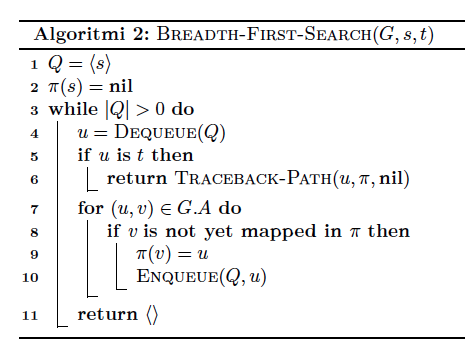
\includegraphics[width=\textwidth,keepaspectratio]{bfs}
\end{figure}
\end{frame}
%%% END: BFS pseudocode

\begin{frame}
Voiko leveyssuuntaisen haun nopeuttaa?
\end{frame}

\begin{frame}
Voi!
\end{frame}

\begin{frame}
\frametitle{Kaksisuuntainen leveyssuuntainen haku}
\begin{itemize}
  \item Ajaa kaksi hakuavaruutta: yksi normaalin tapaan lähtösolmusta, ja toinen ''takaperin'' maalisolmusta.
  \item Kun kaksi yllä mainittua hakuavaruutta kohtavat jossain ''keskellä'', rakennetaan lyhin polku.
  \item Aikavaativuus on $2\sum_{i = 0}^{\lceil N / 2\rceil} d^i$.
  \item Verkosta riippuen voi olla jopa \textasciitilde 1000 kertaa nopeampi kuin yksisuuntainen BFS.
\end{itemize}
\end{frame}

\begin{frame}
\begin{figure}[H]
  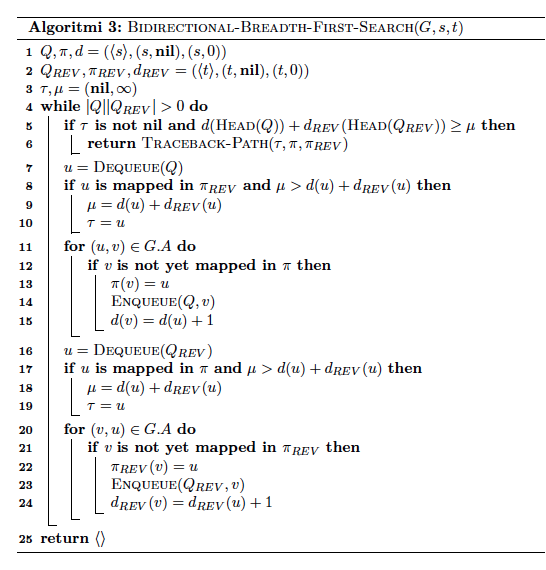
\includegraphics[width=\textwidth,height=\textheight,keepaspectratio]{bibfs}
\end{figure}
\end{frame}

\begin{frame}
Miten rakentaa polut lyhimpien polkujen puusta?
\end{frame}

\begin{frame}
Tarvitaan vain kuvaus $\pi$ (ja myös $\pi_{REV}$ mikäli polku oli haettu kaksisuuntaisella haulla).
\end{frame}

\begin{frame}
  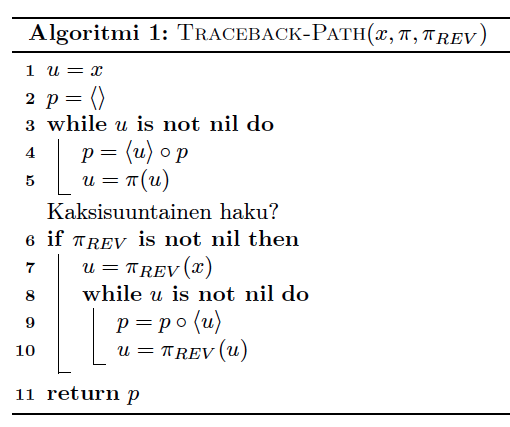
\includegraphics[width=\textwidth,height=\textheight,keepaspectratio]{path}
\end{frame}

\begin{frame}
  \frametitle{Dijkstran algoritmi}
  \begin{itemize}
    \item Vuonna 1959 Edsger W. Dijkstra esitti kuuluisan polunhakualgoritminsa, joka käy polynomisessa ajassa.
    \item LIFO jonon sijasta prioriteettijono; kutsutaan usein ''avoimeksi'' listaksi (engl. \textit{open set}).
    \item Hajautustauluun perustuva joukkorakenne; kutsutaan usein ''suljetuksi' listaksi (engl. \textit{closed set}).
    \item $g$-kuvaus, joka kuvaa kunkin saavutetun solmun toistaiseksi pienempään etäisyyteen lähtösolmusta laskettuna.
    \item $\pi$-kuvaus, aivan kuten BFS:ssä (kuvaa solmun edeltäjäänsä lyhimpien polkujen puussa).
    \item Kun solmu poistetaan avoimesta listasta, sen $g$-arvo on optimaali. $a \circ b$
  \end{itemize}
\end{frame}

\begin{frame}
  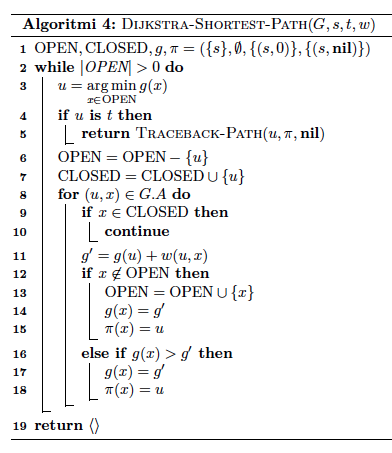
\includegraphics[width=\textwidth,height=\textheight,keepaspectratio]{dijkstra}
\end{frame}

\end{document}